%\documentclass[a4paper, 12pt]{report}
\documentclass[12pt,a4paper,openany]{abntex2}

\usepackage[T1]{fontenc}
%\usepackage[latin1]{inputenc}
%\usepackage[verbose,left=30mm,right=20mm,top=30mm,bottom=30mm]{geometry}
%\usepackage{txfonts}
\usepackage[brazil]{babel}
\usepackage{pdfpages}
%\usepackage[authoryear]{natbib}
%\usepackage{appendix}
%\usepackage{setspace}
%\usepackage{url}
%\usepackage{hyperref}
%\usepackage{color}
\usepackage[utf8]{inputenc}
\usepackage{placeins}
\usepackage{float}

\autor{Leonardo Mendonça de Araujo \and \\ Lucas Bagatini do Nascimento \and \\ Mário Muramatsu Júnior}
\titulo{RELATÓRIO DE FINAL: IDENTIFICADOR DE SINAIS TRIFÁSICOS}
\data{2018} 
\local{Rio Claro, São Paulo}
\preambulo{Monografia apresentada ao curso de Ciências da Computação, como requisito parcial para a obtenção do Título de Bacharel em Ciências da Computação, Instituto de Geociências e Ciências Exatas da Universidade Estadual Paulista}
\orientador{Mario Roberto da Silva}
\tipotrabalho{monografia}

\begin{document}
	
\imprimircapa	
\imprimirfolhaderosto

\clearpage
\cleardoublepage
\cleardoublepage

\pagenumbering{arabic}
\setcounter{page}{3}

\tableofcontents
\clearpage{\pagestyle{empty}\cleardoublepage}
	
\chapter{Materiais e Metodologia}

  Para a etapa de projeto conceitual e virtual dos módulos do circuito foi utilizado
o software Quartus na sua versão 9.0 com licença universitária.
  Constituindo as funcionalidades do Quartus temos a área de trabalho do projeto,
em que podem ser arrastados elementos de hardware como portas lógicas, pinos de
entrada e saída, flip-flops, fios, barramentos e muito mais.
  Além da área de trabalho temos a opção de fazer alterações nos componentes do
circuito por meio do uso de HDL (Linguagem de Descrição de Hardware), e também é
possível executar testes funcionais e/ou de tempo para verificar a integridade dos
módulos desenvolvidos antes de testá-los na placa física.
  A Figura ~\ref{fig:interface-quartus} mostra a interface do usuário do Quartus versão 9.0.

%Figura X (interface-quartus)
\begin{figure}[!htp]
	\centering
	\fbox{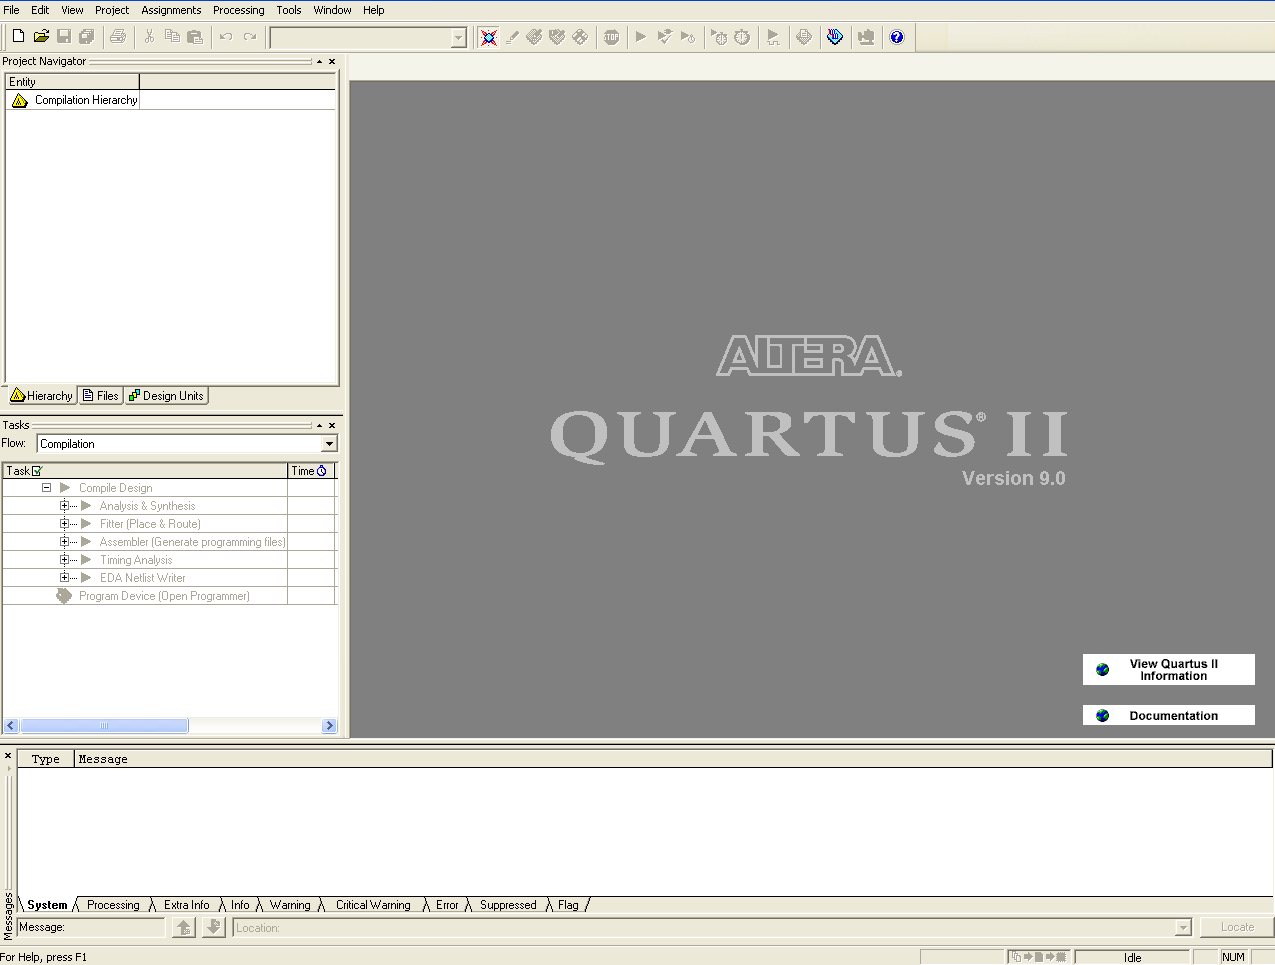
\includegraphics[width=16cm]{images/interface-quartus.png}}
		\caption{Interface do Programa Quartus}
	\label{fig:interface-quartus}
\end{figure}

\section{NOME DA SEÇÃO}

  Juntamente com o software Quartus versão 9.0, foi usada para o desenvolvimento e teste
de todas as etapas do projeto a placa UP Educational Board, que está representada
detalhadamente pela Figura ~\ref{fig:placa-1}.

%Imagem da placa_1
\begin{figure}[!htp]
	\centering
	\fbox{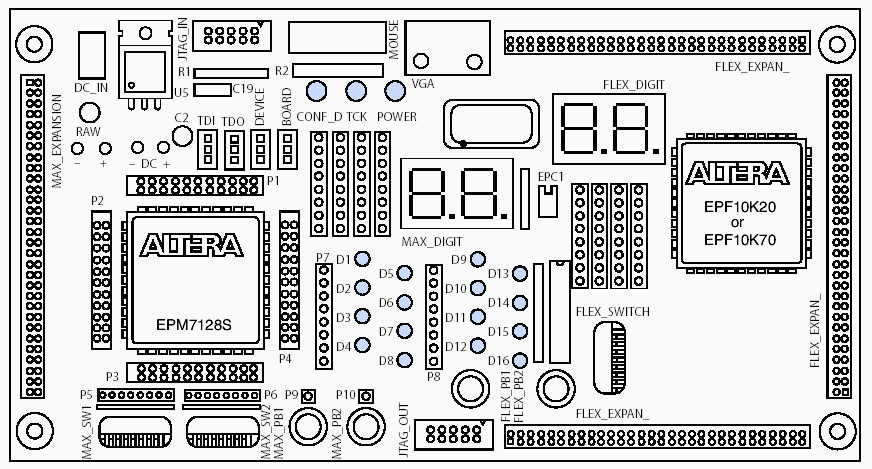
\includegraphics[width=16cm]{images/placa_1.png}}
		\caption{Overview da Placa}
	\label{fig:placa-1}
\end{figure}

  Alguns dos elementos da placa usados para a simulação do funcionamento dos módulos
foram os pinos de entrada e saídas de led para identificar saídas do circuito.

* Explicar necessidade do Antibouncing
\section{NOME DA SEÇÃO}

  Quando trabalhamos com um circuito que envolve entradas mecânicas (como a ponta de prova),
tem-se o surgimento de um efeito conhecido como “bouncing”.
  Esse efeito é caracterizado por “idas” e “vindas”, do nível lógico alto e o nível
lógico baixo, antes de efetivamente estabilizar. Essas oscilações rápidas podem
gerar acionamentos indevidos no nosso circuito. Pois o mesmo tende a interpretar
que a ponta de prova foi acionada repetidas vezes em um curto espaço de tempo,
quando na verdade foi apenas uma vez.
  Devido a isso, foi necessário o desenvolvimento de um módulo de Antibouncing
integrado ao sistema para lidar com o problema. Usando técnicas de desenvolvimento
de máquinas sequenciais conseguimos que o sinal de entrada similar ao da imagem A
fosse manipulado, gerando uma saída como o apresentado na imagem B.

%Imagem A (sinal com bouncing)
\begin{figure}[!htp]
	\centering
	\fbox{\includegraphics[width=16cm]{images/????.png}}
		\caption{Sinal com Bouncing}
	\label{fig:sinal-com-bouncing}
\end{figure}

%//Imagem B (sinal sem bouncing)
\begin{figure}[!htp]
	\centering
	\fbox{\includegraphics[width=16cm]{images/????.png}}
		\caption{Sinal sem Bouncing}
	\label{fig:sinal-sem-bouncing}
\end{figure}

* Explicar necessidade do Timeout
\section{NOME DA SEÇÃO}

  Após ser implementado o módulo de AntiBouncing, o grupo se deparou com uma nova
situação problemática, foi identificado que o sinal capturado pela ponta de prova
(podendo ser R, S ou T), como já era esperado, começava a se defasar com o passar
dos segundos, no entanto, depois de um período específico essa defasagem tornava-se
tão severa que o sinal já não podia mais ser identificado como R,S ou T.
  Esse período foi chamado de período de Timeout do sinal obtido pela ponta de prova
e foi necessário o desenvolvimento de um módulo adicional integrado ao sistema que
fosse capaz de cronometrar esse período e que identificasse quando um sinal contido
na entrada da ponta de prova seria confiável ou não.
  Se identificado o sinal não-confiável seria necessário a obtenção de um novo sinal
por meio do acionamento da ponta de prova, tendo novamente um sinal aceitável para
ser manipulado novamente pelos outros módulos do circuito.


%----------------Exemplo: insere figura-----------------------
%\begin{figure}[!htp]
%	\centering
%	\fbox{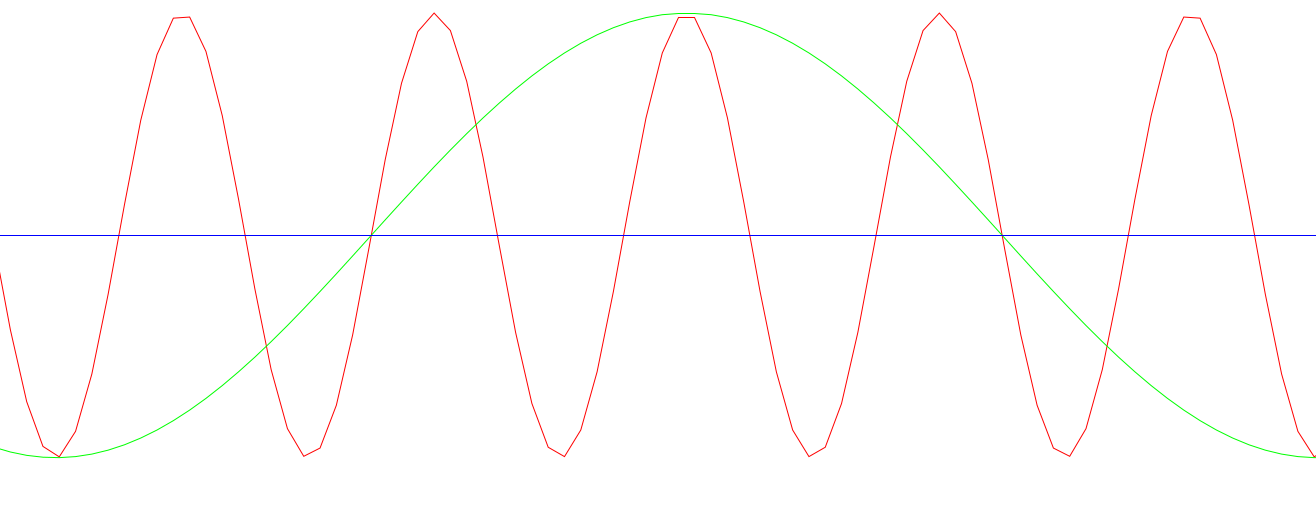
\includegraphics[width=16cm]{images/ondas.png}}
%		\caption{Exemplo de ondas sonoras}
%	\label{fig:ondas-sonoras}
%\end{figure}

%---------------Exemplo: insere tabela -----------------------
%\begin{table}[h]	
%	\centering	
%	\vspace{0.5cm}	
%\begin{tabular}{r|lr}
%Notas  & Frequ{\^e}ncia (Hz) \\
%\hline 
%C (Dó) & 261,33          \\
%D (Ré) & 293,66          \\
%E (Mi)  & 329,63 		 \\
%F (Fá)  & 349,23 		 \\
%G (Sol) & 391,99 		 \\  
%A (Lá)  & 440,00  		 \\
%B (Si)  & 493,88
%\end{tabular}
%	\label{tab:frequencia-notas}
%	\caption{Frequência da notas centrais do piano}
%\end{table}

\end{document}
